\graphicspath{{dp/figures/}}
\chapter{X-ray Total Scattering Data Acquisition and Processing} \label{ch:dp}
\section{Introduction}
X-ray total scattering experiments are generally performed at synchrotron light sources, as only these sources can provide the needed flux, energy, and high momentum transfer vectors needed to obtain reliable PDFs. \cite{Chupas2003, Dykhne2011}
Despite the need for a dedicated facility to perform the total scattering experiments, the experiments themselves are fairly forgiving, allowing for reactive gaseous environments, experiment temperatures ranging from 2 \si{K} to 1800 \si{K}, and even electrochemical cycling. \cite{Chupas2008, Petkov2013, Redmond2012}
The rapid PDF data acquisition associated with 2D area detectors creates a data management problem, as 96 hours of beamtime could result in almost $10,000$ images which need to be associated with the experimental conditions and detector metadata. \cite{Chupas2003}
 Finally, all this data needs to be processed by masking bad pixels and regions, integrating azimuthally, and converting the scattering data to the PDF. \cite{Kieffer2013, Juhas2013, Yang2014, Pauw2014, Billinge2012}

%\section{Data Storage and Management}

Processing the raw pixel intensities to the PDF is very important as we are extracting most of our interesting information out of very high $Q$ data.
This data relies on good statistics and sound background subtraction.
Talk about papers from Billinge Group with thin film PDF and dilute NP solutions.
Diagram of the overall data processing workflow.
Discuss the NSLS-II data stack.
\begin{figure}
\centering
\begin{tikzpicture}[thick,scale=0.6, every node/.style={scale=0.6}]
    \node (img) [startstop] at (0,0) {Image Data};
    \node [database, right=of img] (fs)  {FileStore};
    \node[startstop, below=of img] (imeta) {Image Metadata};
    \node[startstop, below=of imeta] (emeta) {Environmental Metadata};
    \node[startstop, below=of emeta] (bmeta) {Beamline Metadata};
    \node[startstop, below=of bmeta] (smeta) {Sample Metadata};
    \node[database, right=of emeta] (mds) {MetadataStore};
    \node[process, right=of mds] (db) {DataBroker};
%     \node[io, right=of db] (lfg) {Load Data};
%     \node[io, below=of lfg] (lbg) {Load Background};
%     \node[process, right=of lfg] (maskfg) {Mask Data};
%     \node[process, right=of lbg] (maskbg) {Mask Background};
%     \node[process, right=of maskfg] (ifg) {Azimuthally Integrate Data};
%     \node[process, right=of maskbg] (ibg) {Azimuthally Integrate Background};
%     \node[process, right=of ifg] (bgsubs) {Subtract Background};

%     \draw[->] (img) -- ++(0,1) -- ++($(fs)+(0,1)$)node[] -- (fs);
%     \draw[->] (F)--(Z) node [midway,above] {$\Sigma$};
%     \draw[->] (M)--(N) node [midway,below] {$\psi'$};
%     \draw[->] (E)--(M) node [midway,left] {$\phi$};
%     \draw[->] (N)--(Z) node [midway,left] {$\tilde{\phi}\Sigma$};
\end{tikzpicture}
\caption{Database Loading Workflow. Data is loaded from various sources, including images and text files, into the FileStore and MetadataStore databases. Data is then retrieved from the databases using the databroker.}
\end{figure}
\subsection{MetadataStore Side Loading}
Design of sidewinder-spec for loading the data into metadatastore.
Most of the design considerations went into the loaders, which are different for each experiment.

\subsection{Detector $Q$ resolution} \label{subsec:qres}
To properly azimuthaly integrate the images taken from the detector the $Q$ resolution of the pixels must be calculated.
Integrating using even bins will cause pixels which are not on the same ring to be binned together, causing the incorrect value of $I(Q)$ to be obtained and a larger standard deviation in the integrated data.
To properly calculate the $Q$ resolution the resolution of each of the pixels in $2\theta$ must be calculated.
\begin{figure}
    \centering
    \begin{tikzpicture}
        \draw (0,0) node[anchor=north]{$A$}
          -- (4,0) node[anchor=north]{$C$}
          -- (4,4) node[anchor=east]{$B$}
          -- cycle;
        \draw (0,0) node[anchor=north]{$A$}
          -- (4,0) node[anchor=north]{$C$}
          -- (4,6) node[anchor=south]{$B'$}
          -- cycle;
    \end{tikzpicture}
    \caption{Scattering onto a flat detector}
    \label{fig:scattering_digram}
\end{figure}
Figure \ref{fig:scattering_digram} shows the scattering of x-rays onto a flat image plate detector.
In this diagram the bottom of the $n$th pixel is $B$ while the top is $B'$.
The resolution of this pixel in $2\theta$ is $\angle BAC - \angle B'AC$.
Thus the resolution, calculated from the distances is
\begin{equation}
\Delta 2 \theta = \arctan{\frac{b}{d}} - \arctan{\frac{t}{d}}
\end{equation}
where d is the sample to detector distance, b is the distance to the bottom of a pixel, and t is the distance to the top of that pixel.
Note that these distances need to have been corrected for detector tilt and rotation.
Thus the resolution of a pixel in $Q$ is
\begin{equation}
\Delta Q = \frac{4\pi(\sin{\arctan{\frac{b}{d}}} - \sin{\arctan{\frac{t}{d}}})}{\lambda}
\end{equation}
where $\lambda$ is the x-ray wavelength.

For a Perkin Elmer image plate, like the one used at the NSLS-II's XPD and the APS's 11-ID-B, the resolution function is shown in \ref{fig:res_func}.
For the same detector the number of pixels per $Q$ is shown in \ref{fig:pixel_hist}
\begin{figure}[!ht]
  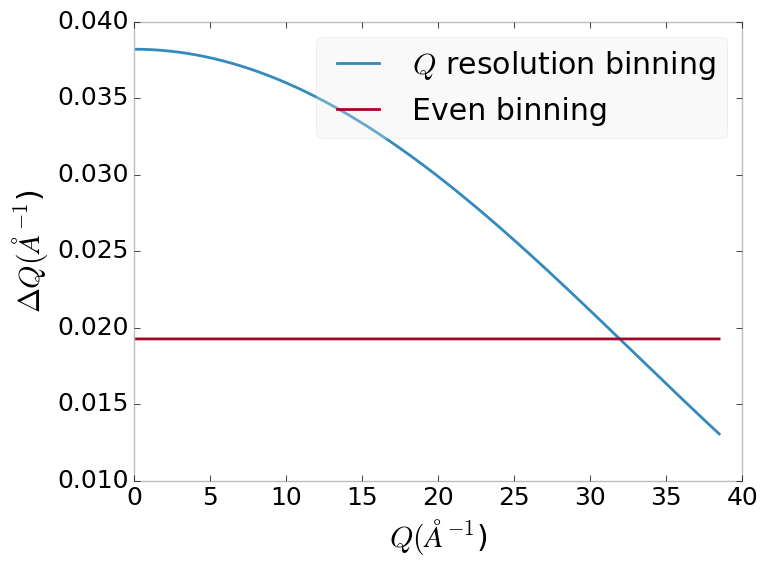
\includegraphics[width=\textwidth]{res}
\caption{$Q$ resolution as a function of $Q$.}
\label{fig:res_func}
\end{figure}

\begin{figure}[!ht]
  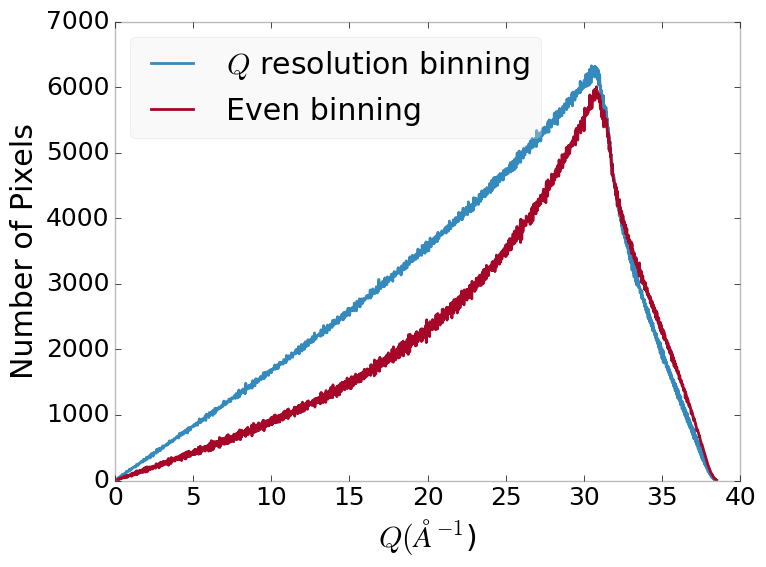
\includegraphics[width=\textwidth]{pixels}
\caption{Number of pixels as a function of $Q$, binned at the $Q$ resolution of the detector.}
\label{fig:pixel_hist}
\end{figure}

\section{Automated Mask Generation} \label{subsec:mask}
\subsection{Introduction}
Detector masking is an important part of any x-ray scattering workflow as dead/hot pixels, streak errors, and beamstop associated features can be averaged into the data changing the signal and its statistical significance.
While some features, like the beamstop holder, can be easily observed and masked by hand other are much more difficult to observe even on large computer monitors.
Additionally, while dead/hot pixels and streaks are usually static the hot pixels associated with textured or single crystal scattering or cosmic rays are not.
Thus, coming up with an automated method for finding such erroneous pixels is important, especially as high flux diffraction beamlines can generate data very quickly.

While this problem can be quite complex in the most general case, we can use the annular symmetry of the powder scattering pattern to our advantage, by comparing a pixel against pixels in the same ring.
Since non-textured powder scattering should produce the same pixel intensity for a given ring we can mask any pixels which are $\alpha$ standard deviations away from the mean.
This method relies on the aforementioned pixel binning algorithm, as using miss sized bins will cause some pixels which should be in separate rings to be put together, and others which should be in the same ring to be separated.
In that case the masking algorithm will overestimate the number of pixels to be masked due to the additional statistical variation in the sample.

\subsubsection{Algorithm Design}
The masking algorithm procedure takes in the image and a description of the pixel positions in either distance from the point of incidence or in $Q$.
The image is then integrated twice, producing both the mean $I(Q)$ and the standard deviation of each $I(Q)$ ring.
The mask is created by comparing the pixel values against each ring's standard deviation and threshold $\alpha$.
Note that the threshold can be a function of distance from the point of incidence or $Q$.

\subsubsection{Test Cases}
To study the effectiveness of the masking we ran the algorithm against both simulated experimental data.
In the case of the simulated data four systems were created:
1) dead/hot pixels with varying numbers of defective pixels,
2) beamstop holder with varying beamstop holder transmittance,
3) rotated beamstop holder with varying beamstop holder transmittance,
and 4) beamstop holder with dead/hot pixels.
The base scattering was produced by
\begin{equation}
I = 100\cos(50r)^{2} + 150
\end{equation}
where $r$ is a pixel's distance from the beam point of incidence.
The positions of the dead/hot pixels were chosen at random as was the dead or hot nature of the defect. Dead pixels had values from 0 to 10, while hot pixels had values from 200 to 255.
The beamstop was positioned at the vertical center of the detector with an initial width of 60 pixels and final width of 120 pixels.
The height of the beamstop was 1024 pixels.
The beamstop was calculated to attenuate the x-ray scattering signal at various transmittance, as various beamstop holder materials have different transmittance.
Two version of the masking algorithm were run for each test case, one using the standard even bin sizes for the integration step, and one where the bin sizes are tuned to the pixel $Q$ resolution as discussed in \ref{subsec:qres}.

\subsubsection{Results and Discussion}
\foreach \n in {100, 300, 500, 1000}{
\begin{figure}
  \centering
  \foreach \m in {masked}{
    \subfloat[]{\includegraphics[width=.5\textwidth]{bad_bin_dead_pixel_\m_\n}}
    \subfloat[]{\includegraphics[width=.5\textwidth]{dead_pixel_\m_\n}}
    }
\caption[Generated dead/hot pixel masks for a detector with $\n$ bad pixels.]{Generated dead/hot pixel masks for a detector with $\n$ bad pixels. a) the standard even bin mask and b) the $Q$ resolution binned mask. The bad pixels are noted with open circles, masked pixels are noted with closed circles.}
  \label{fig:dead_pixel_\n}
\end{figure}
}

\foreach \n in {10, 30, 50, 90}{
\begin{figure}
  \foreach \m in {raw, masked, missed}{
    \subfloat[]{\includegraphics[width=.3\textwidth]{\m_\n}}
    }
  \caption[Generated beamstop holder masks for a beamstop holder with $\n\%$ transmittance.]{Generated beamstop holder masks for a beamstop holder with $\n\%$ transmittance. a) the raw image, b) the masked image, c) and the missed pixels}
  \label{fig:bs_\n}
\end{figure}
}

\begin{figure}
        \foreach \m in {raw, masked, missed}{
        \subfloat[]{\includegraphics[width=.3\textwidth]{rotate_\m_50}
        }}
    \caption{Generated beamstop holder masks which is rotated away from vertical}
    \label{fig:rot_bs}
\end{figure}

Figures \ref{fig:dead_pixel_100}-\ref{fig:bs_90} show the results of the masking algorithm on simulated images.
The dead/hot pixel masking shows the importance of using the $Q$ resolution based bin sizes as the even bin based mask have a tendency to over mask the image, removing pixels which contain valuable signal.
This over-masking is caused by pixels being improperly associated with one another by the even bins.
Figure \ref{fig:dead_pixel_100} indicates that the masking algorithm, with the proper binning, masks the image perfectly, with no missed bad pixels or good pixels masked.
This is not the case in figures \ref{fig:dead_pixel_300} - \ref{fig:dead_pixel_1000} as we can see pixels which should have been masked but were not.
Despite these missed pixels no pixels were improperly masked in any of the well binned images.
These test cases are actually more difficult than experimental data, as the dynamic range of most detector causes the dead/hot pixels and single crystal/texture peaks to be orders of magnitude away from the desired signal.

The beamstop holder masks shown in figures \ref{fig:bs_10} - \ref{fig:bs_90}, which were all run with the $Q$ resolution binning show similar results across the transmittance range, missing only a small part of the beamstop holder near the point of incidence.
Near this point the beamstop holder becomes a statistically significant part of the total number of pixels in a given ring, thus it can not be masked out using a statistical search of the rings.
For most PDF and XRD studies this small area can be masked automatically by masking all the pixels who's distance from the point of incidence is smaller than a given radius $r$, or can be neglected outright as the area is not used in the analysis or refinement.
Similar results were produced for beamstop holders which were rotated away from the vertical position, as shown in figure \ref{fig:rot_bs}

\begin{figure}
    \foreach \m in {raw, masked}{
        \subfloat[]{\includegraphics[width=.5\textwidth]{exp_\m}}
    }
    \caption[Masked experimental data.]{Masked experimental data. a) the raw image, b) the mask}
    \label{fig:masked_exp}
\end{figure}

\begin{figure}
    \foreach \m in {raw, masked}{
        \subfloat[]{\includegraphics[width=.5\textwidth]{single_xtal_\m}}
    }
    \caption[Masked experimental data with Pt single crystal signal.]{Masked experimental data with Pt single crystal signal. a) the raw image, b) the mask}
    \label{fig:masked_single_xtal}
\end{figure}

\begin{figure}
    \foreach \m in {raw, masked}{
        \subfloat[]{\includegraphics[width=.5\textwidth]{combined_\m}}
    }
    \caption[Masked experimental data with Pt single crystal signal using figure's \ref{fig:masked_exp} mask as a starting mask.]{Masked experimental data with Pt single crystal signal using figure's \ref{fig:masked_exp} mask as a starting mask. a) the raw image, b) the mask}
    \label{fig:combined}
\end{figure}

Working with actual experimental data, obtained at the Advanced Photon Source beamline 11-ID-B, shows the difficulty of masking images which have low photon counts.
While the masking of experimental data taken with longer exposures, consisting of 250 .2 second shots, shown in figure \ref{fig:masked_exp} provides very sharp edges to the beamstop holder, and very little extra masking beyond the occasional dead pixel, this is not the case for the single crystal data.
The single crystal data is more problematic because of its short exposure time and low flux, with 500 frame at a .1 second exposure and having shrunk the beam size.
The low flux is to prevent the very strong single crystal peaks from damaging the detector.
However, this causes the image to be less statistically viable then ideal, causing problems with the mask as seen in figure \ref{fig:masked_single_xtal}.
This can be alleviated to some degree by using the previously generated mask as a starting mask for the single crystal image, as shown in \ref{fig:combined}.
While the masking algorithm still produces many diffuse masked pixels, they are far fewer, this may be due to the removal of the beamstop which could have contributed to the large standard deviation in figure \ref{fig:masked_single_xtal}.


\subsubsection{Conclusions}
In this section the masking algorithm, which relies on both $Q$ resolution based binning and a statistical approach to azimuthal symmetry, was developed.
The focus of this algorithm was to remove many unwanted detector features associated with pixel defect, beamstop holder associated scattering attenuation, and single crystal/texture peaks.
Simulated data was used to evaluate the beamstop holder and dead/hot pixel masking capacity, while experimental data was used to check for single crystal and texture based masking.
$Q$ resolution based binning was shown to be very important to avoid over-masking.
The ability of the mask writer to mask images is somewhat limited by the overall statistical image quality, although some deficiencies can be obtained by using previously generated masks as starting points.
This masking algorithm is now in use in the data processing workflow and will be available in scikit-beam soon.


\section{Automated Image Azimuthal Integration} \label{subsec:int}
Using the $Q$ resolution binning and masking developed in sections \ref{subsec:qres} and \ref{subsec:mask} the images can be properly integrated.
Generally, images are integrated by taking the mean value of the pixels in a ring.
However, other statistical measures of the average value can be used, like the median.

Figures \ref{fig:workflow_no_mask}-\ref{fig:workflow_auto_mask} show the importance of masking and the choice of average function.
All the figures were produced using the same dataset, 50 \si{\degree}C \ce{Pr2NiO4} taken at the APS's 11-ID-B on a Perkin Elmer area detector.
The automatic masking alpha was $3$ standard deviations from the mean.
While it is difficult to observe the changes the mask causes in the full $I(Q)$ plot (subfigures a) and b)), the standard deviation plots show the effect of bad pixels on the data (subfigure c)).
Subfigure c) for figures \ref{fig:workflow_no_mask}-\ref{fig:workflow_auto_mask} shows that removal of the beamstop holder lowers the low $Q$ standard deviation from around .1 to almost .01 out to 15 \iA.
The high $Q$ subfigures d) and f) in figures \ref{fig:workflow_no_mask}-\ref{fig:workflow_auto_mask} show the ``kink'' effect of the detector edge and beamstop holder, where there is a dip in the $I(Q)$ scattering when the rings include the edge of the detector.
This effect seems to be due to both errors in the edge pixel intensity and the beamstop holder as masking of the edges only seems to provide only partial removal of the issue.
It is important to note that while integration using the mean of the ring has issues with only the edge mask, as evidenced by the change in slope in \ref{fig:workflow_edge_mask} d) around 29.5 \iA, the median integration does not include this error.
Ideally the detector would have a normal distribution of pixel intensity for a given ring, which would imply an equivalency between the mean and median $I(Q)$ values.
Despite the closeness of the mean and median once the final mask has been created, it seems that the median is more reliable, as it was less effected by the beamstop holder in figure \ref{fig:workflow_edge_mask}.
Thus, for subsequent integrations discussed in this work the median is used to avoid any defective features that the masking algorithm may have missed.

%\begin{landscape}
\foreach \n/\o in {no_mask/with no mask, edge_mask/with only an edge mask, auto_mask/combining an edge mask and the automatically generated mask}{
    \begin{figure}[!h]
    \centering
    \foreach \m in {img, mask, ave, std, high_q_ave, high_q_std}{
        \subfloat[]{\includegraphics[width=.4\textwidth]{\n_\m}}
        }
    \caption[Masking, average, and standard deviation of an example x-ray total scattering measurement with \o.]{Masking, average, and standard deviation of an example x-ray total scattering measurement. This image was produced \o. a) the image, b) the mask, c) the mean and median values, d) the standard deviation (normalized to the median), e) a closeup of the 28 \iA to 31 \iA $Q$ range for the mean and median, f) 28 \iA to 31 \iA $Q$ range for the standard deviation}
    \label{fig:workflow_\n}
    \end{figure}
}
%\end{landscape}

\section{Conclusions}
This chapter developed and analyzed the proper data processing and reduction methodology for producing reliable $F(Q)$ data from x-ray total scattering measurements.
Binning at the $Q$ resolution of the detector was found to be key to the data processing.
The primary outcome of using the $Q$ resolution binning was an enhancement in effectiveness for the masking algorithm, producing much fewer false positives for dead/hot pixels.
This masking approach was then applied to the integration of experimental data taken at the APD's 11-ID-B beamline.
The automatically generated masks, when combined with edge masks, were found to greatly reduce the overall standard deviation of the pixel intensity and produce a smoother $F(Q)$ at high $Q$, enabling the use of much higher $Q$ data in the PDF.
Different statistical measures used in the azimuthal integration was also compared.
This comparison showed that the median was a more reliable statistic for integration with data which had more detector defects.
However, upon properly masking it was shown that these metrics were almost identical.
The masking induced similarity between the mean and median shows that the rings, when integrated, may form a Gaussian distribution.
The distribution of the pixel intensities for strongly and weakly scattering samples may be investigated in future work.